\documentclass[11pt,a4paper]{article}
\usepackage[margin=1in]{geometry}
\usepackage[T1]{fontenc}
\usepackage[utf8]{inputenc}
\usepackage{lmodern}
\usepackage{hyperref}
\usepackage{enumitem}
\usepackage{xurl}
\usepackage{tikz}
\usepackage{float}
\usetikzlibrary{arrows.meta, positioning, shapes.geometric}
\hypersetup{colorlinks=true,linkcolor=blue,urlcolor=blue}
\newcommand{\codepath}[1]{\path{#1}}
\tikzset{box/.style={rectangle,draw,rounded corners,align=center,inner sep=3pt,minimum width=36mm},line/.style={-Latex}}

\title{Phase-1 Deliverable: Baseline Adapter}
\author{SIT Engine Architecture}
\date{\today}

\begin{document}
\maketitle

\section{Technical Description}
Baseline Adapter is the reference ingest path used to validate deterministic end-to-end pipeline behavior before specialized adapters are introduced.

\section{Implementation Fulfillment}
Implemented in \codepath{Phase-1/adapters/baseline_adapter.py}, with raw CPU parsing delegated to \codepath{Phase-1/adapters/cpu_adapter.py}. CLI integration occurs in \codepath{Phase-1/cli.py} via \texttt{cmd\_ingest}.

\section{Design \& Architecture}
Baseline adapter supports both normalized CSV and raw trace paths, applies ingest validators, and writes deterministic trace/residency artifacts plus manifest metadata.

\subsection*{Function Flowchart}
\begin{figure}[H]
\centering
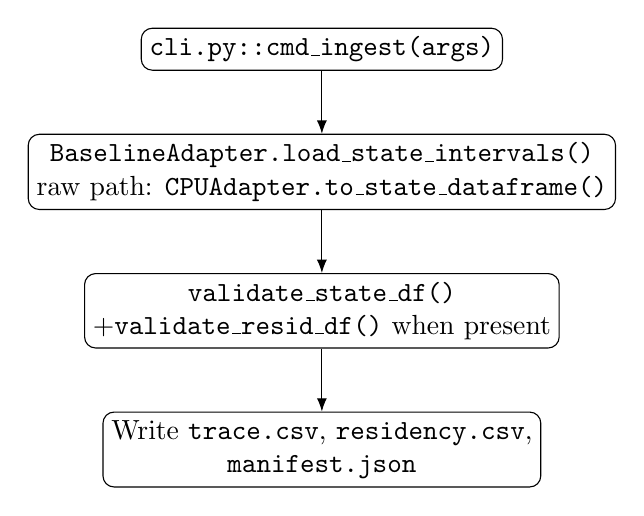
\begin{tikzpicture}[node distance=8mm and 12mm]
\node[box] (a) {\texttt{cli.py::cmd\_ingest(args)}};
\node[box, below=of a] (b) {\texttt{BaselineAdapter.load\_state\_intervals()}\\raw path: \texttt{CPUAdapter.to\_state\_dataframe()}};
\node[box, below=of b] (c) {\texttt{validate\_state\_df()}\\+\texttt{validate\_resid\_df()} when present};
\node[box, below=of c] (d) {Write \texttt{trace.csv}, \texttt{residency.csv},\\\texttt{manifest.json}};
\draw[line] (a) -- (b);
\draw[line] (b) -- (c);
\draw[line] (c) -- (d);
\end{tikzpicture}
\caption{Baseline Adapter Function Flow}
\end{figure}

\end{document}
